\section{Aufgabe 2}
In dieser Aufgabe Soll der Frequenzgang an 3 Lastwiderständen gemessen werden. Diese könnten z.B. Lautsprecher repräsentieren, die jeweils Wechselstrom mit verschiedenen Frequenzen in Schallwellen umwandeln können. Gemessen wird also die Effektivspannung am Funktionsgenerator \(U_G\) und die jeweiligen Effektivspannungen an den Lastwiderständen \(U_i\). 
\subsection{Aufbau}
Um sich den Aufbau besser vorstellen zu können hier das Schaltbild:
\begin{center}
\begin{minipage}{\linewidth}
\centering
\makebox[0cm]{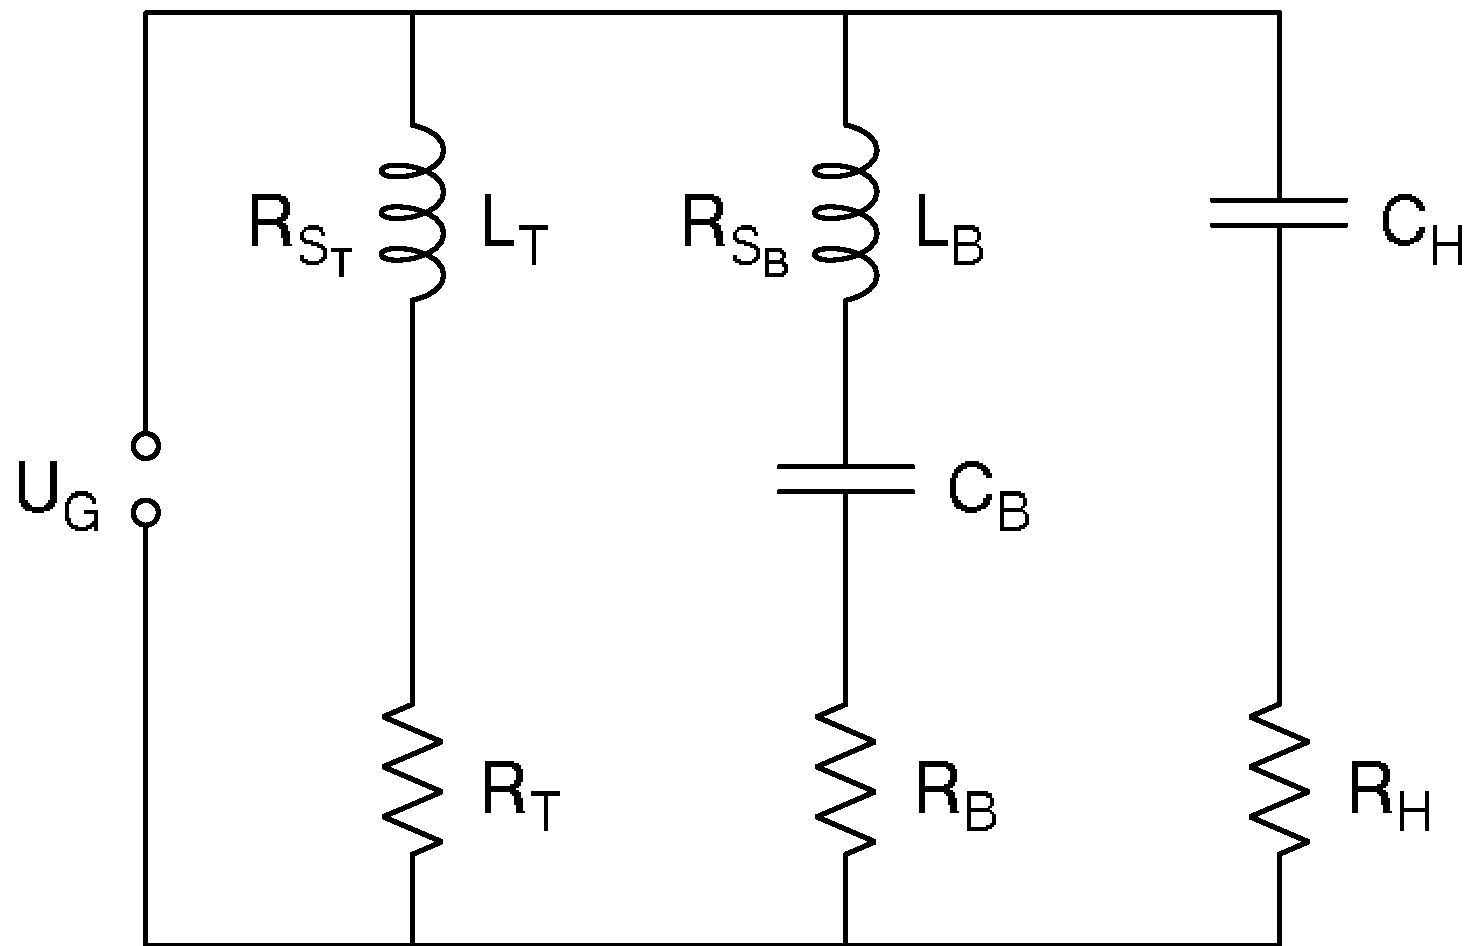
\includegraphics[width=10cm]{frequenzweiche}}
\captionof{figure}{Schaltplan der Frequnzweiche}%
\label{frequenzweiche_schaltplan}
\end{minipage}
\end{center}
Die Einzelnen Komponenten wurden auf ein Steckbrett aufgesteckt und mit Steckbrücken und Bananensteckern verbunden.
\begin{center}
\begin{minipage}{\linewidth}
\centering
\makebox[0cm]{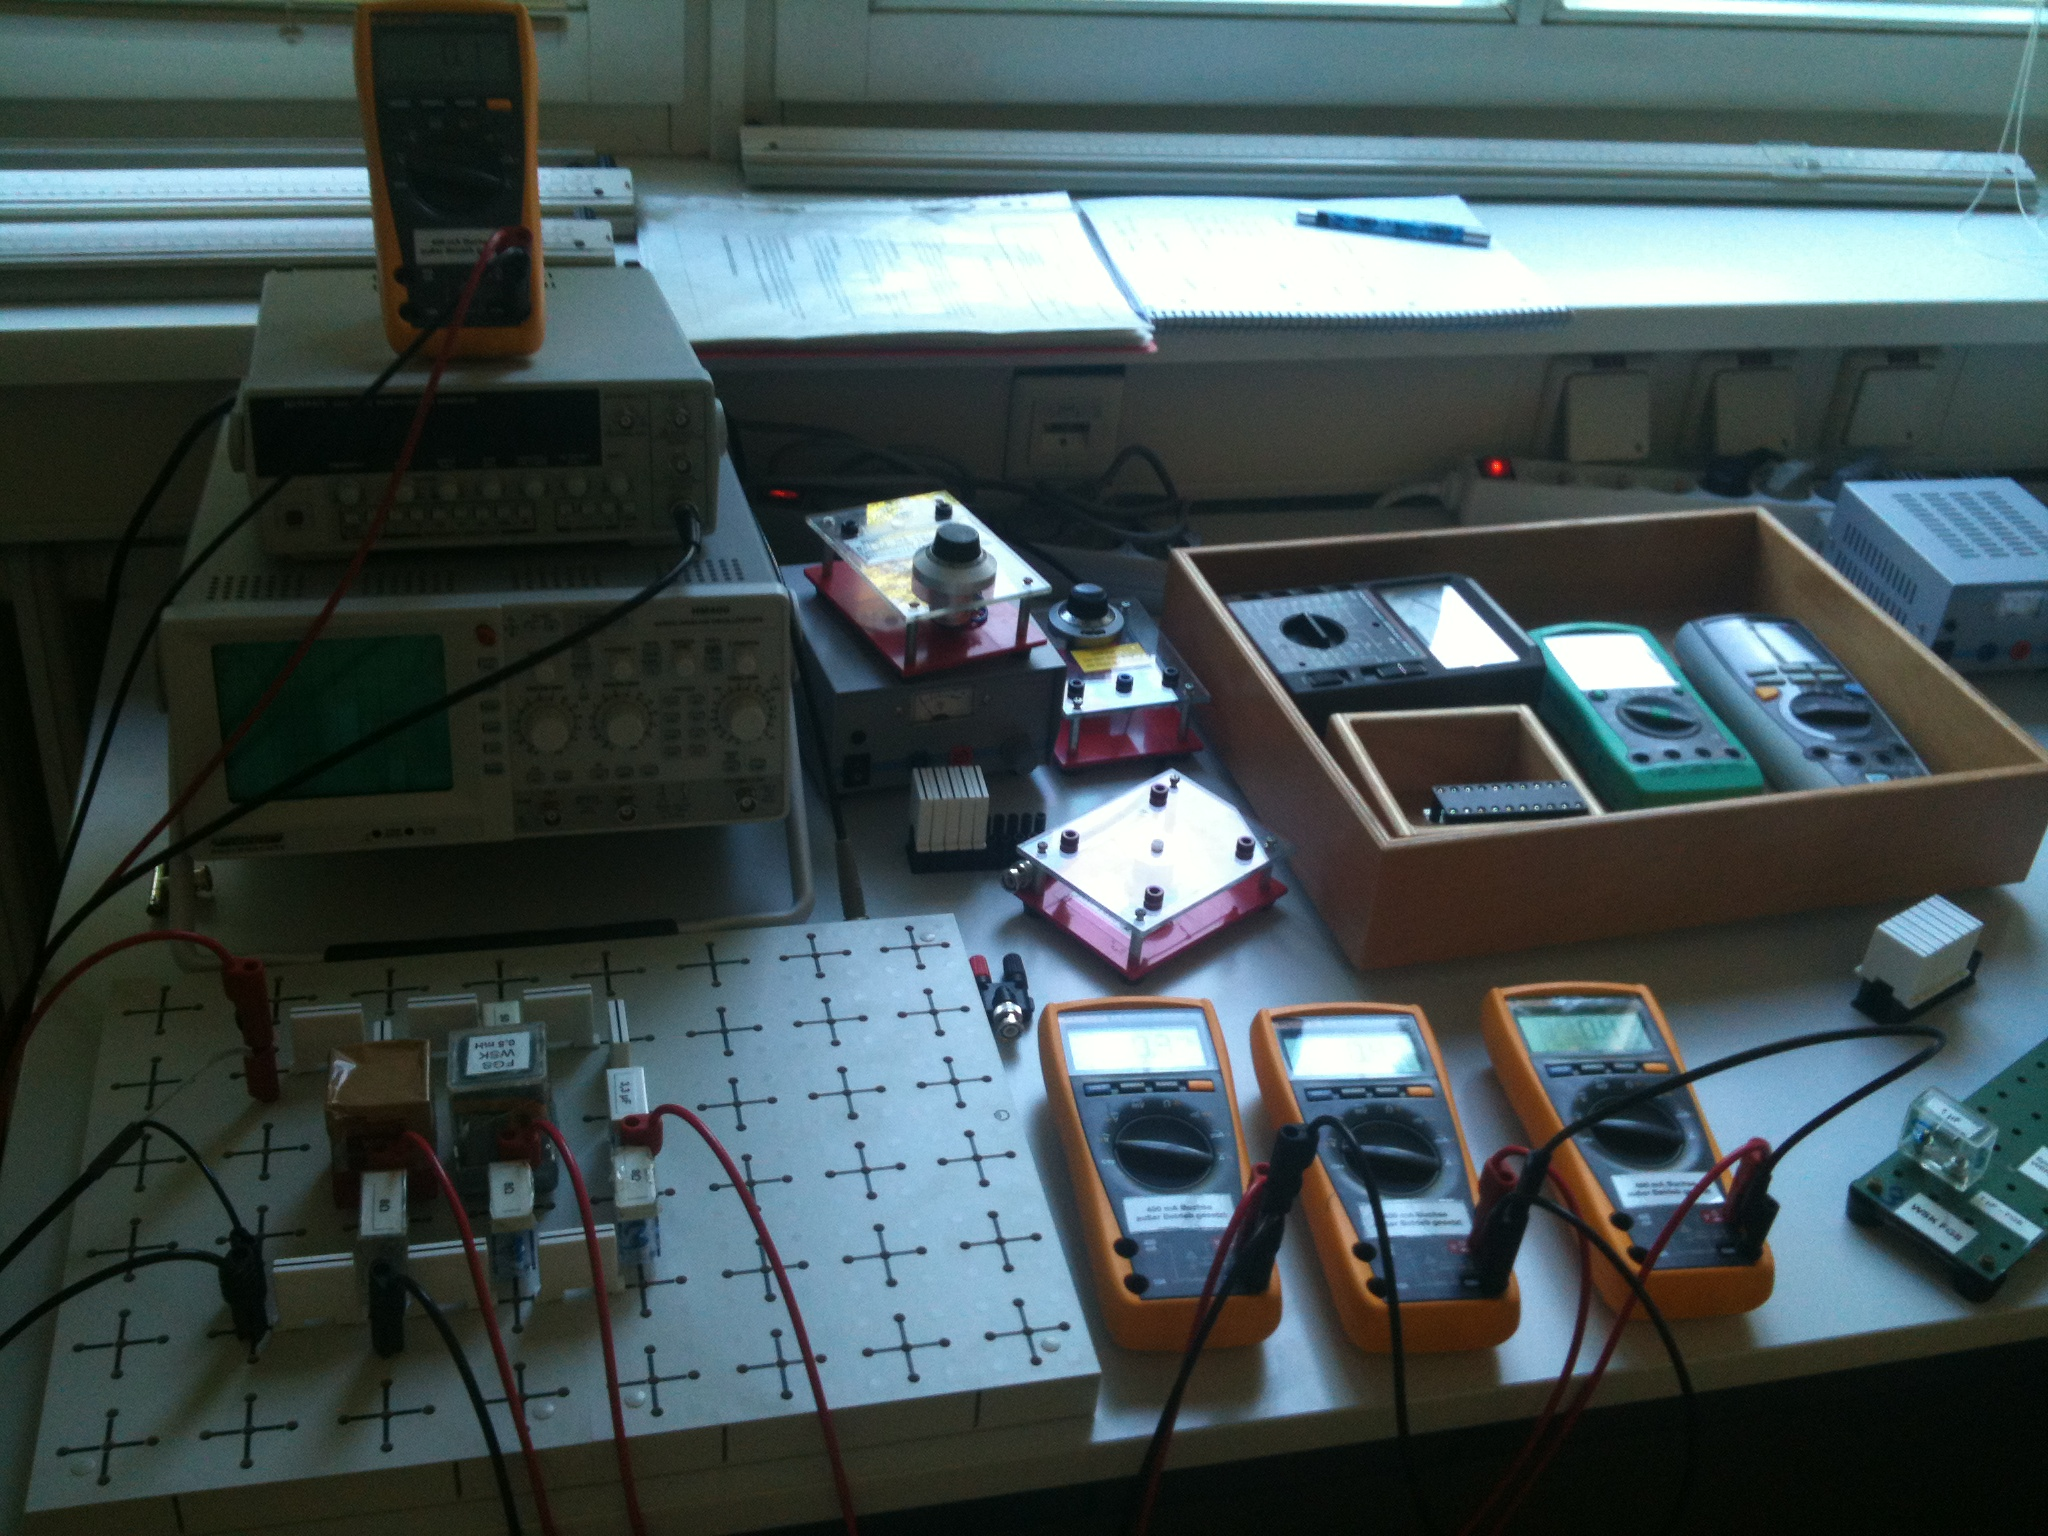
\includegraphics[width=\textwidth]{Bilder/IMG_0027}}
\captionof{figure}{Der Versuchsaufbau}%
\label{frequenzweiche_aufbau}
\end{minipage}
\end{center}
\subsection{Gegebenes}
Um im Anschluss die Messwerte einordnen zu können, wurden folgende Daten separat gemessen:
\begin{center}
\begin{tabular}{c|c}
Messgröße & Messwert\\\hline
\(R_{S_T}\) & \(\left(3,7 \pm 0,5 \right)\, \Omega \) \\
\(L_T\) & \((4,823\pm 0,063)\, mH \) \\
\(R_T\) & \((8,46\pm 0,11)\, \Omega \) \\
\(R_{S_B}\) & \(\left(1,0 \pm 0,5 \right)\, \Omega \) \\
\(L_B\) & \((487\pm 10)\, \mu H \) \\
\(C_B\) & \((38,08\pm 0,32)\, \mu F \) \\
\(R_B\) & \((8,10\pm 0,11)\, \Omega \) \\
\(C_H\) & \((3,172\pm 0,027)\, \mu F \) \\
\(R_H\) & \((8,06\pm 0,11)\, \Omega \) \\
\end{tabular}
\captionof{table}{Sepperate Messung}%
\end{center}
Die Widerstände der Spulen wurden dabei mit dem Voltcraft VC230 gemessen, Kapazitäten, Induktivitäten und die Widerstände der Lastwiderstände hingegen mit dem ELC-131D.
\subsection{Messwerte}
TODO Tabellen
\subsection{Auswertung}
\subsection{Graphische Auftragung}
\begin{center}
\begin{minipage}{\linewidth}
\centering
\makebox[0cm]{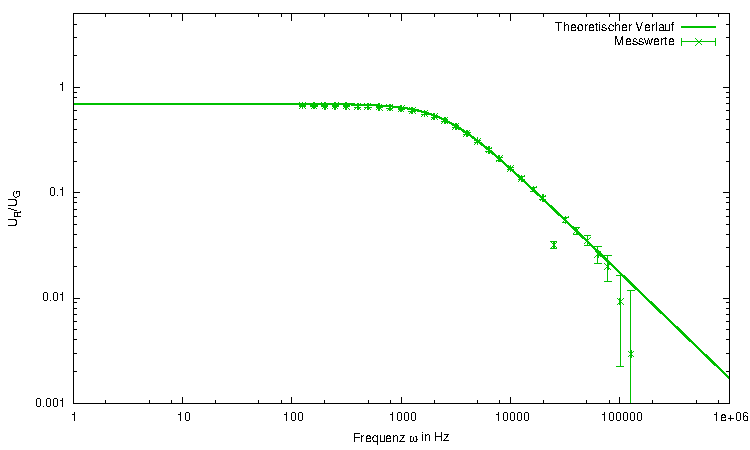
\includegraphics[width=\textwidth]{graphen/tiefpass}}
\captionof{figure}{Messung am Tiefpass}
\end{minipage}
\begin{minipage}{\linewidth}
\centering
\makebox[0cm]{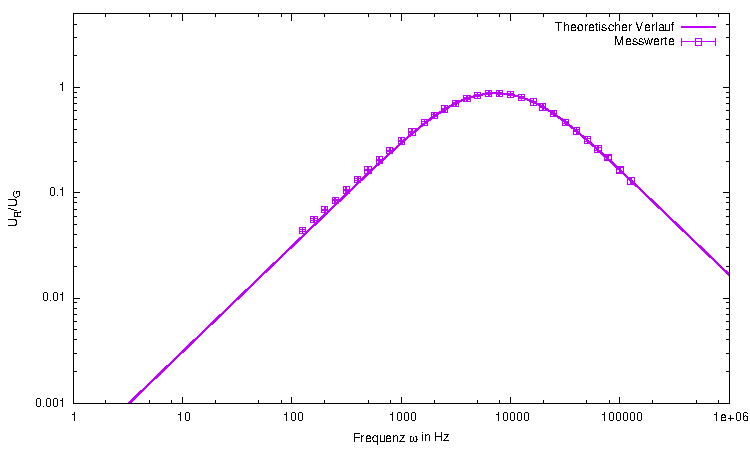
\includegraphics[width=\textwidth]{graphen/bandpass}}
\captionof{figure}{Messung am Bandpass}
\end{minipage}
\begin{minipage}{\linewidth}
\centering
\makebox[0cm]{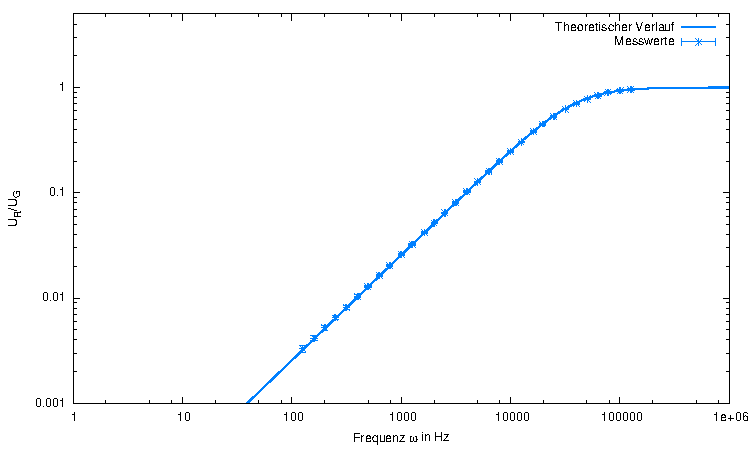
\includegraphics[width=\textwidth]{graphen/hochpass}}
\captionof{figure}{Messung am Hochpass}
\end{minipage}
\end{center}
\subsection{Fazit}